%\section{Web Operating System Simulator as an Evidence in the Teaching-Learning Process}
\section{OS Simulator within a Syllabus of Web Programming}
\label{sec:GralExplanation}
Regardless of the methodology used, in a course, a syllabus must be covered.
We propose a project that has given us very good results and that we have been polishing 
for the last 9 years. Our proposal is to develop a Web-based Operating System Simulator.
Next sections explain how the integrator project is adapted with the syllabus and the
evaluation.

\subsection{Learning Units}
\label{ssec:learningUnits}
Below we describe the learning units that students should receive during the course.
The subject comprises 16 weeks, each week involves 3 face-to-face hours and 
3 extra-class hours. Our restriction is to provide in a single course web 
programming topics of Front-end and Back-end, hence we have conformed the 
following units: 
i) Design, development and programming of web pages on the client's side; 
ii) Internet, WWW and HTTP; and 
iii) Programming of server-side web pages.

The first unit comprises three learning outcomes: 
i) Design web pages on the client side using HTML5 and CSS3 technologies;
ii) Develop programs that involve the use of the programming language on the 
client side (JavaScript) and relate it to HTML and CSS; and 
iii) Know different JavaScript Technologies (e.g. jQuery) and frameworks used 
in the design phase (e.g. Boostrap).

The second unit comprises: 
i) Describe the historical perspective of the Internet, the family of 
TCP/IP protocols, as well as WWW; 
ii) Know the Client/Server architecture focusing and detailing the operation 
of the HTTP protocol; 
iii) Install web servers and database.

The third unit includes: 
i) Identify existing technologies for server-side web programming; 
ii) Know the paradigm of web programming on the server side (session variables, 
cookies, ajax, etc.); 
iii) Develop programs using a server-side language.

With these three units we cover the main topics and try not to saturate the students.

\subsection{OS Simulator as a Project Integrator and Teaching Strategy}
\label{ssec:projectIntegrator}

Thinking about a final project where students can start and expand in terms of design 
and development is not an easy task. As previously mentioned, our proposal is to 
develop a Web-based Operating System Simulator. This involves for 
the student to choose an existing Operating System to replicate it in terms of design, 
and to develop some modules so that a simulation is actually reached in terms of 
operability. 

This proposal is divided into two phases: design and development (Units 1 and 3 in 
Section~\ref{ssec:learningUnits}). 
The design phase involves the initial project with Front-end themes such as HTML, 
CSS and JavaScript. 
The development phase involves the final project and is specified when back-end 
technologies have already been taught such as server installation (Unit 2 in 
Section~\ref{ssec:learningUnits}) and server-side programming. 
In both phases, practices are carried out that lead to the synergy of the initial 
project (respectively the final one).

\subsection{Evidence of Learning}
Teaching programming courses in general is difficult, and web programming is not the 
exception. Deciding what kind of activities and projects will be used in a course of 
these, as well as achieving a good balance between the theoretical part and the 
practice, is quite difficult. Here we propose seven evidences; classified in two: 
a) Know; and 
c) Skills. 
Each of them has been assigned a specific percentage with respect to the 
general score of the course (See Table~\ref{table:learningEvidences}).

% Please add the following required packages to your document preamble:
% \usepackage{multirow}
\begin{table}
    \begin{center}
        \caption{General evidences proposal}
        \label{table:learningEvidences}
        \begin{tabular}{|l|l|l|}
        \hline
        \multicolumn{1}{|c|}{\multirow{2}{*}{Knowledge:35\%}} & Middle Exam                   & 15\% \\ \cline{2-3} 
        \multicolumn{1}{|c|}{}                           & Final Exam                    & 20\% \\ \hline
        \multirow{5}{*}{Skills:65\%}                     & Client side Practices         & 10\% \\ \cline{2-3} 
                                                         & Server side Practices         & 10\% \\ \cline{2-3} 
                                                         & Client-Server Practices       & 10\% \\ \cline{2-3} 
                                                         & Initial project specification & 15\% \\ \cline{2-3} 
                                                         & Final project specification   & 20\% \\ \hline
        \end{tabular}
    \end{center}
\end{table}    


Students must necessarily obtain at least (70/100) as a general average of all evidence 
to pass the course. Throughout the delivery of this teaching-learning method, a 
difficulty has been identified by reaching 100\% of the final grade. To combat this 
restriction and taking into account the students' inspiration, two strategies have 
been promoted so that they can obtain an extra grade. On the one hand, the practical 
challenges and on the other hand, the participation, attendance and participation in 
extracurricular activities.

Figure~\ref{fig:evidences} shows a summary of the evidences distributed throughout a 
course. To have a balance we have divided it into four blocks. As you can see in the red 
box, the Development of the Operating System Simulator covers the entire course. 
You can also notice how the exams are outside the development of the Simulator, and this 
is obvious because in these evidences theoretical contents are evaluated, in some way 
what is sought is that the development of the simulator is a support to reach the 
theoretical and practical knowledge.

\begin{figure}[bt]
 %\begin{center}
  \centering
    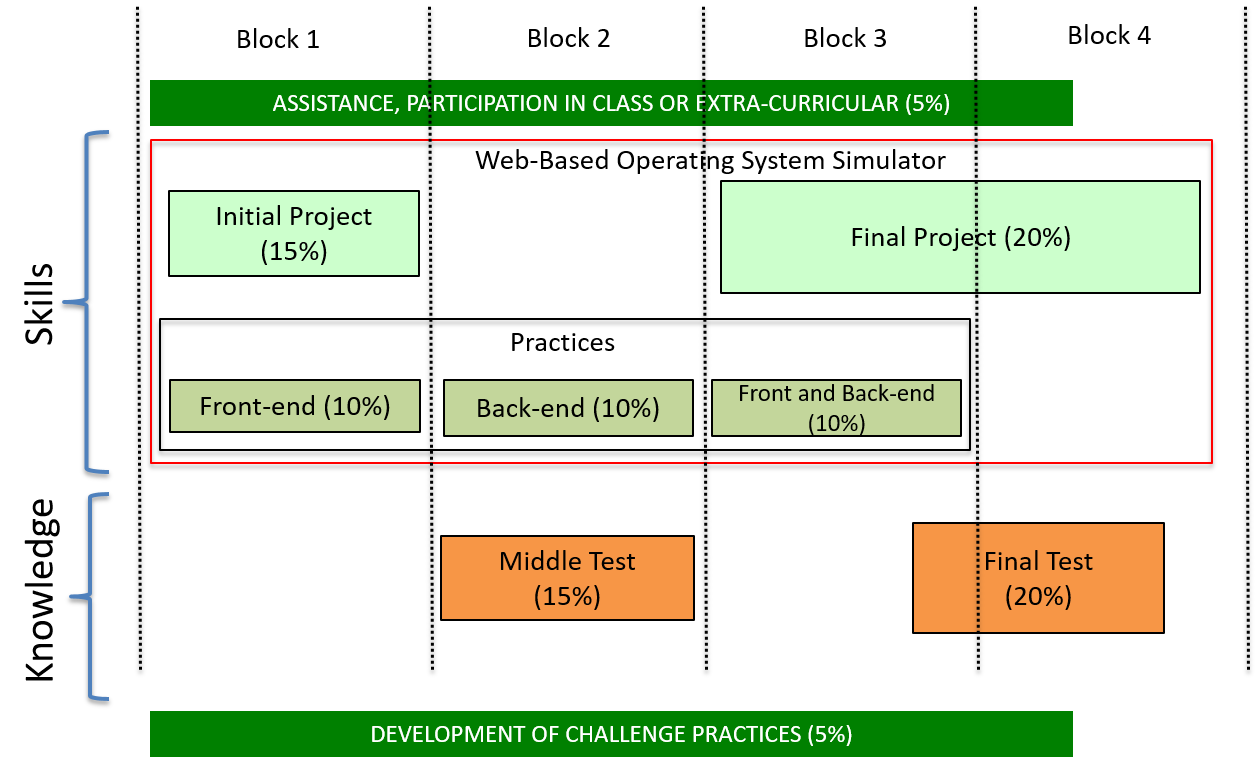
\includegraphics[scale=0.6]{images/evidence.png}
    \caption{Graphical description of all evidences applied in all the course of web programming }
    \label{fig:evidences}
 % \end{center}
\end{figure}
